\documentclass[11pt,a4paper]{article}
\usepackage[margin=2.2cm]{geometry}
\usepackage[T1]{fontenc}
\usepackage{lmodern,microtype,amsmath,amssymb,graphicx,booktabs,caption,tabularx,xcolor,float,setspace,lineno}
\usepackage[numbers,sort&compress]{natbib}
\providecommand{\bibcommenthead}{}
\usepackage[hidelinks]{hyperref}
\usepackage{orcidlink}
\captionsetup{font=small,labelfont=bf}
\newcommand{\cj}[1]{{\color{blue!60!black}[CJ: #1]}}   % CJ's review comments; collected with grep '\\cj{' and removed before submission
\setlength{\parskip}{0.3em}
\renewcommand{\topfraction}{0.9}\renewcommand{\bottomfraction}{0.6}\renewcommand{\textfraction}{0.05}\renewcommand{\floatpagefraction}{0.85}
\newcommand{\pending}[1]{{\color{red!70!black}[#1]}}   % results still being acquired or identifiers to mint; removed before submission
\onehalfspacing


\title{Supplementary Information\\ \large The page is already a lattice: historical objects as native registers on neutral-atom quantum processors}
\author{Christophe Jurczak\,\orcidlink{0009-0001-8204-7333}\\ \normalsize Metamorphoses of Civilization Collection, Dallas, TX, USA\\ \normalsize Quantonation, Dallas, TX, USA\\ \normalsize Correspondence: \href{mailto:christophe@quantonation.com}{christophe@quantonation.com}}
\date{}

\begin{document}
\maketitle
\renewcommand{\thesection}{S\arabic{section}}
\renewcommand{\thetable}{S\arabic{table}}

\noindent Equation and figure numbers refer to the main text; the references are listed at the end.


\section{The objects: background}
Until the nineteenth century a book was printed from movable type set by a compositor into formes. Corrections were often made while a forme was on the press, so early sheets carry the uncorrected text and later ones the corrected text, and every surviving copy is a different mixture; such stop-press variants are found by comparing copies letter by letter, as Hinman did for the First Folio with an optical collator~\cite{hinman1963}. Libraries now publish high-resolution images of many copies of the same edition, which is why such pages, already arrays of discrete units at near-uniform pitch, are a natural input for an atom array.

The \emph{Eucharisticos} of Paulinus of Pella (616 hexameters, about 459) rests on two witnesses, the 1579 Paris edition of Marguerin de La Bigne~\cite{labigne1579} from a manuscript since lost, and Bern, Burgerbibliothek, Cod.~317; every modern edition combines them~\cite{brandes1888,moussy1974,lucarini2006}. Our collation of nine copies shows the print corrected at press forme by forme. On the page carrying columns 287--288 (signature m6v), line 314, the corrector removed the final \emph{s} of \emph{omnis} without re-spacing the line (Figure~1e,f of the main text); the uncorrected state, which agrees with the Bern manuscript, survives in two of the nine copies (P$^1$, one in the author's collection), the corrected in seven (P$^2$). The First Folio (London, 1623~\cite{shakespeare1623}) is used through the Bodleian copy Arch.~G~c.7 (CC-BY 3.0 IIIF images, 5412$\times$7216 pixels) and two copies at the University of Pennsylvania, with Rizvi's transcription~\cite{rizvi} and the compositor attributions compiled by Blayney~\cite{blayney1996} as per-page metadata.

\section{The mosaic generator}
The generator produces tessera lattices on square or hexagonal packings at unit pitch with three kinds of break: dislocations, where a row of tesserae ends and the rows on either side close over it; figure seams, where tesserae following a curved course meet the background courses; and edges. Patches hold 20--80 tesserae. Dislocation density and course curvature were set so that the per-tessera neighbour-count distribution matched that measured on segmented panels of Roman pavements (segmentations in the repository); the generator models the break, not its cause. The two families of the main text, G1 and G3, differ in packing and break density; their 100 and 101 windows are in the repository with per-tessera labels.

\section{Bond-dimension convergence}
A window is converged at a readout time if the mean $|\Delta\langle n_i\rangle|$ between adjacent rungs of the ladder is below 0.005 and the mean nearest-neighbour $|\Delta C_{ij}|$ below 0.002. For the \emph{Eucharisticos} windows (67--77 atoms) occupations change by 0.005 on average (0.04 at most) between $\chi=300$ and 600, the locus contrasts strengthen by about 10\% in the same direction, and no ranking changes; $\chi=600$ values are quoted. On three 95-atom Folio blocks the emulation converges at 1\,$\mu$s but is still changing at 4\,$\mu$s in five of six block--regime cases (mean $|\Delta\langle n_i\rangle|$ up to 0.074). On the 38--60-atom synthetic windows (\S S4) the criterion is met on all 20 windows only to $Jt=2$, on 14 of 20 from $Jt=4$ to 60.

The registers of Figure~4 were emulated at $\chi=150$, 300, 600 and 1000 with 24 readout times, and a precision-limited run ($10^{-6}$, $\chi\le1600$) recorded the half-register entanglement entropy. Table~\ref{tab:e1} gives, per register, regime and adjacent pair of rungs, the last readout time to which the criterion holds, and the entropy at 6\,$\mu$s. Registers of 23--37 atoms are converged to 6\,$\mu$s; the 56-atom die-link register is converged under the AFM drive and to 1.25\,$\mu$s under the FM-like one (its middle-cut entropy is zero because no blockade pair straddles the cut); the 73-atom corrected window converges to 6 and 4.5\,$\mu$s; the 76-atom uncorrected window and the 93-atom mosaic leave the criterion between 0.1 and 3\,$\mu$s at every rung. The one-body Spearman between the 1000-shot hardware occupations and the $\chi=600$ profile at every time is in the repository (\texttt{fig2\_hw\_curves.json}); the medians over the sixteen emulated times are 0.98 (FM-like) and 0.62 (AFM) for the 37-atom Folio window, 0.96 and 0.62 for the side-note window, 0.85 and 0.42 for the corrected window, 0.80 and 0.50 for the uncorrected one, 0.59 and 0.37 for the mosaic, 0.52 and 0.56 for the die links. The hardware's mean occupation relative to the emulated one is 1.05--1.13 (AFM) and 1.12--1.29 (FM-like) on the converged registers, up to 1.8 and 2.7 on the unconverged ones (\S S11). Against the classical rate-equation model of \S 3.3 of the main text, driven by the interaction descriptors and the lattice counts, the per-window correlation between the hardware residual and the emulator residual on 24 fresh Folio windows is $+0.75$ under the FM-like drive, positive in 24 of 24 windows (none of 2000 permutations reached the observed median, $p<5\times10^{-4}$); under the AFM drive it is $-0.09$ (10 of 24 windows positive): no agreement beyond the rate model.

\begin{table}[h]
\centering\small
\caption{Bond-dimension ladder at the Figure~4 operating point: last converged readout time $t^*$ ($\mu$s) for each adjacent pair of rungs, and mean $|\Delta\langle n_i\rangle|$ at 6\,$\mu$s in parentheses. $S$, half-register entanglement entropy at 6\,$\mu$s from the precision-limited run.}
\label{tab:e1}
\begin{tabular}{llrlllr}
\hline
register & regime & $N$ & 150/300 & 300/600 & 600/1000 & $S$ \\
\hline
Folio window & AFM & 37 & 3.5 (0.006) & 5.5 (0.006) & 6.0 (0.003) & 6.7 \\
Folio window & FM & 37 & 2.0 (0.012) & 3.5 (0.007) & 6.0 (0.003) & 3.4 \\
side-note window & AFM & 29 & 6.0 (0.000) & 6.0 (0.000) & 6.0 (0.000) & 3.6 \\
side-note window & FM & 29 & 6.0 (0.001) & 6.0 (0.000) & 6.0 (0.000) & 3.4 \\
generated mosaic & AFM & 23 & 6.0 (0.000) & 6.0 (0.000) & 6.0 (0.000) & 3.8 \\
generated mosaic & FM & 23 & 6.0 (0.001) & 6.0 (0.000) & 6.0 (0.000) & 1.7 \\
die links & AFM & 56 & 2.0 (0.022) & 2.0 (0.020) & 6.0 (0.001) & 0 (cut) \\
die links & FM & 56 & 1.6 (0.030) & 1.25 (0.024) & 1.25 (0.017) & 0 (cut) \\
\emph{Eucharisticos}, corrected & AFM & 73 & 2.0 (0.005) & 3.0 (0.004) & 6.0 (0.003) & 6.5 \\
\emph{Eucharisticos}, corrected & FM & 73 & 2.5 (0.009) & 3.0 (0.006) & 4.5 (0.003) & 1.8 \\
\emph{Eucharisticos}, uncorrected & AFM & 76 & 0.1 (0.013) & 0.1 (0.012) & 0.1 (0.027) & 6.7 \\
\emph{Eucharisticos}, uncorrected & FM & 76 & 0.1 (0.014) & 4.0 (0.006) & 0.1 (0.005) & 1.8 \\
real mosaic & AFM & 93 & 0.85 (0.011) & 1.0 (0.009) & 1.35 (0.013) & 6.6 \\
real mosaic & FM & 93 & 4.5 (0.004) & 4.0 (0.004) & 3.0 (0.005) & 1.8 \\
\hline
\end{tabular}
\end{table}

\section{The synthetic cycle-parity test}
Figure~\ref{fig:syn1} shows the paired AUROC against readout time at both gates. At the first gate (10--18 atoms, exact evolution, 50 pairs) the quench features read the parity (0.99 at $Jt=50$), but so did the local descriptors (0.75--0.82): on the triangular lattice an induced cycle has only $120^\circ$ corners, so the number of corners is even and the parity of $L$ equals the parity of the number of straight sites, whose $r^{-6}$ fields differ from those of corners. The leak falls as $1/L$, and the quench residual beyond the local descriptors (0.82--0.89) is already reached from 1-hop clusters (0.78--0.85): the same leak, read nonlinearly. The gate was repeated at a size where the leak must vanish.

\begin{figure}[h]
\centering
\includegraphics[width=0.95\textwidth]{figures/syn1_range.png}
\caption{The range of the quench features on the synthetic cycle-parity task: paired AUROC against readout time $Jt$. (a) Gate 1, 10--18 atoms, exact evolution: full-window quench features (raw and residual beyond the local descriptors) and the same residual from 1-hop truncated dynamics; the band is the local-descriptor score. (b) Gate 2, 38--60 atoms, emu-mps at $\chi=300$ (60 windows) and $\chi=600$ (20 windows): full-window features, residual, and residual from 2- and 4-hop truncated dynamics; dashed, the 0.90 reference line. The $\chi=300$ curve is converged only to $Jt\approx3$.}
\label{fig:syn1}
\end{figure}

At the second gate (38--60 atoms, 30 pairs, $L=31$--48) the local descriptors are blind (paired AUROC 0.34 and 0.45 under the two learners on all 60 windows, 0.08 and 0.07 on the 20-window $\chi=600$ subset). Values below 0.5 arise in paired cross-validation at 30 pairs, where held-out predictions anti-correlate with the training fit; a pair-respecting permutation test confirms it: with the parity label flipped within a random half of the pairs (200 permutations, the same learners) the null 95\% interval is 0.24--0.72 under the linear learner and 0.28--0.74 under the boosted one, and the observed values lie inside it (one-sided $p=0.12$ and 0.32). RRWP is blind below $K=31$ except by 0.03 and perfect at odd $K>48$. The quench features reach at best 0.73, at $Jt=12$ on the 60 windows ($\chi=300$) and at $Jt=30$ on the $\chi=600$ subset, against the 0.90 rule; 0.73 sits at the upper edge of its own permutation null (0.27--0.76, $p=0.05$ before the choice of $Jt$ among twenty readout times is accounted for). What separation exists (0.78 on the 60 windows) is reproduced by 2-hop truncated dynamics (0.77 at $r=2$, 0.69 at $r=4$). At $Jt\le150$ the quench features do not resolve a global parity, as the bound of \S 2.3 of the main text leads one to expect (\texttt{synthetic/permutation\_syn1g2\_chi300.json}).

\section{Readout-phase witness}
The register is a (3,5) facilitation interferometer of 10 atoms whose ten bonds are resonant at $r^*=7\,\mu$m and whose non-bonded pairs are at least 11.2\,$\mu$m apart. The facilitation pulse has $\Omega_f=3.0$\,rad/$\mu$s and $\delta_f=C_6/r^{*6}=7.36$\,rad/$\mu$s for 2000\,ns, then a pause of 340\,ns identical for both phases, then a readout pulse of area $\pi/2$ at the amplitude cap ($\Omega=15.104$\,rad/$\mu$s, 104\,ns, $\delta=0$) at phase $\varphi=0$ or $\pi/2$ relative to the drive; 10 repetitions of each phase, 1000 shots per row. The drift control (first against last five repetitions at fixed phase) shows no drift. The one-body witness is positive on 8 of 10 sites with one common sign, contrasts $+0.018$ to $+0.036$ (standard error 0.007), about half the $0.037$--$0.056$ predicted by the September noise model (\S S11); the two-body witness is null on 0 of 10 bonds, contrasts $-0.006$ to $+0.004$ against a predicted $0.023$--$0.030$ (Figure~\ref{fig:t3}). This is a contrast at one time, not a decay-rate measurement.

\begin{figure}[h]
\centering
\includegraphics[width=0.95\textwidth]{figures/t3_witness.png}
\caption{Readout-phase coherence witness on Ruby (10 atoms, 2\,$\mu$s facilitation, 10 repetitions $\times$ 1000 shots per phase). (a) One-body contrast $\langle n_i\rangle_{\varphi=0}-\langle n_i\rangle_{\varphi=\pi/2}$ on the ten sites, with $\pm3$ standard errors (band), against the design simulation under the device noise model. (b) Two-body contrast $\Delta C_{ij}$ on the ten bonds, same conventions. (c) Drift control: the same contrasts between the first and last five repetitions at fixed phase.}
\label{fig:t3}
\end{figure}

\section{Local addressing: simulation on mosaic patches}
On mosaic patches of 19 tesserae with a coloured figure (exact evolution, AFM quench) a global drive is compared with the same drive plus a detuning proportional to each tessera's colour (Table~\ref{tab:addr}). Where the figure lies in the interior it coincides with the number of neighbours, so the static field already correlates with it; the clean cases are the four patches whose figure lies along the edge. There the global drive's excitation pattern carries geometry only (correlation with the figure $-0.01$ to $+0.30$), while with colour as local detuning the pattern draws the figure ($0.60$--$0.67$) and its outline ($0.50$--$0.71$), and the figure correlation survives removing everything the static field explains ($0.61$--$0.66$).

\begin{table}[t]
\footnotesize
\caption{Local addressing on eight simulated mosaic patches: Pearson correlation of the excitation pattern with the coloured figure. Without addressing (global drive) the pattern does not show the figure; with each tessera's colour encoded as a local detuning it does, including after the part explained by the static field is removed. Edge patches are the clean test, because there the figure does not coincide with the number of neighbours.}
\label{tab:addr}

\begin{tabular}{@{}llccccc@{}}
\toprule
 & & \multicolumn{2}{c}{correlation with the figure} & \multicolumn{3}{c}{local detuning} \\
\cmidrule(lr){3-4}\cmidrule(lr){5-7}
Figure position & Patch & static field $F_6$ & global drive & figure & outline & figure, field removed \\
\midrule
interior & L-shape & $+0.59$ & $-0.37$ & $+0.63$ & $+0.63$ & $+0.57$ \\
 & diamond & $+0.61$ & $-0.12$ & $+0.59$ & $+0.37$ & $+0.32$ \\
 & bar & $+0.42$ & $-0.19$ & $+0.70$ & $+0.70$ & $+0.61$ \\
 & blob & $+0.39$ & $-0.25$ & $+0.52$ & $+0.41$ & $+0.46$ \\
\midrule
edge & top edge & $+0.03$ & $+0.12$ & $+0.64$ & $+0.51$ & $+0.64$ \\
 & left edge & $-0.05$ & $+0.30$ & $+0.60$ & $+0.50$ & $+0.61$ \\
 & corner & $+0.03$ & $-0.01$ & $+0.65$ & $+0.53$ & $+0.65$ \\
 & edge strip & $-0.13$ & $-0.00$ & $+0.67$ & $+0.71$ & $+0.66$ \\
\bottomrule
\end{tabular}
\end{table}

\section{Correlations across an empty line: per-pair values}
\label{sec:si_p3}
The across-cut statistic $S$ of each split block and its matched whole block under the FM-like drive at 6\,$\mu$s, for three independent 1000-shot passes (14--16 November 2026) and pooled to 3000 shots; the null bound is the 95\% interval of $S$ under independent atoms with the observed occupations at the same shot count; pairs numbered as in Figure~2c (\texttt{p3\_river/p3r\_result.json}). Each pass alone gives $S_{\rm whole}>S_{\rm split}$ in 12 of 12 pairs; the split $S$ leaves its own 1000-shot null interval in two passes for pair 4, in one pass for pairs 10 and 12, and in none for the other nine. A post hoc control on the pair geometry: the pseudo-cut of a whole block was matched to its partner by the number of straddling pairs, not by their separations, and about half of a whole block's straddling pairs lie on adjacent lines (slot distance 1 or 2, line distance 1), a class absent from every split block, whose pairs are two or three lines apart. Reweighting each whole block's per-pair contributions to its partner's separation-class proportions (pooled 3000 shots) leaves $S_{\rm whole}>S_{\rm split}$ in 12 of 12 pairs, with the median across filled lines at $7.6\times10^{-4}$ (unweighted $1.0\times10^{-3}$) against $3.6\times10^{-6}$ across empty ones (\texttt{p3\_river/p3r\_reweight.json}). A second control on the residual of the two split blocks that leave the pooled null (pairs 4 and 12): over across-cut pairs at Manhattan slot distance 4--6 the same blocks give $S=6.6$ and $4.1\times10^{-6}$ against a null bound of $1.8\times10^{-6}$, 0.3--0.4 of their near-pair value, where an $r^{-6}$ tail would fall by orders of magnitude between two and four pitches; over the twelve split blocks the far-pair $S$ lies above its null bound in six, median $1.5\times10^{-6}$, and in the whole blocks the far-pair $S$ is 0.1--0.3 of the near one. The residual is a weak block-wide correlation of every pair, consistent with a shot-to-shot variation of the drive or detuning, not the interaction tail (\texttt{p3\_river/p3r\_farpairs.json}).

The readings summarised in \S 3.4 of the main text are as follows. At 95 atoms the hardware can be compared only with an emulation that has not converged (one-body agreement 0.88--0.96 on three Folio blocks under the FM-like drive at 4\,$\mu$s, 0.09--0.64 under the AFM drive; \S S3). Under the FM-like drive at 6\,$\mu$s ($Jt\approx69$) on each of three independent 1000-shot passes: $S_{\rm whole}>S_{\rm split}$ in 12 of 12 pairs ($p=2\times10^{-4}$), AUROC 1.00, median $S$ of $1.0\times10^{-3}$ across a filled line against at most $2\times10^{-6}$ across an empty one, and the split blocks consistent with zero in 10, 12 and 10 of 12. The passes agree block by block (Spearman 0.86--0.96 over the 24 blocks). Pooled to 3000 shots the null interval narrows to $\pm5\times10^{-6}$ and 8 of 12 split blocks remain inside it, short of the 10 of 12 the test asked for; two keep a residual $S$ of $1.4$ and $1.6\times10^{-5}$ and two sit at the bound. The median over the twelve is $3.6\times10^{-6}$ against $1.0\times10^{-3}$: the mean-square correlation across the cut is suppressed by two to three orders of magnitude (a factor 10--30 in amplitude), not to zero. The same ordering holds at 2 and 4\,$\mu$s and under the AFM drive, and on three matched pairs at 44--47 atoms, measured alongside, the hardware $S$ follows the converged $\chi=600$ emulation at Spearman 0.87.

\begin{center}\scriptsize
\begin{tabular}{@{}rrrrrrrr@{}}
\toprule
pair & $S_{\rm split}$ pass 1 & pass 2 & pass 3 & $S_{\rm split}$ pooled & null upper bound, pooled & $S_{\rm whole}$ pooled & whole/split \\
\midrule
1 & $-2.8\times10^{-6}$ & $+10.2\times10^{-6}$ & $-2.9\times10^{-6}$ & $+4.4\times10^{-6}$ & $+4.0\times10^{-6}$ & $1.42\times10^{-3}$ & 321 \\
2 & $+14.5\times10^{-6}$ & $+3.1\times10^{-6}$ & $-2.7\times10^{-6}$ & $+5.2\times10^{-6}$ & $+5.6\times10^{-6}$ & $1.44\times10^{-3}$ & 278 \\
3 & $-4.6\times10^{-6}$ & $+3.4\times10^{-6}$ & $-8.1\times10^{-6}$ & $+1.0\times10^{-6}$ & $+5.4\times10^{-6}$ & $1.01\times10^{-3}$ & 993 \\
4 & $+16.9\times10^{-6}$ & $+6.5\times10^{-6}$ & $+16.7\times10^{-6}$ & $+15.9\times10^{-6}$ & $+4.8\times10^{-6}$ & $1.45\times10^{-3}$ & 91 \\
5 & $+0.6\times10^{-6}$ & $-2.2\times10^{-6}$ & $+9.4\times10^{-6}$ & $+3.2\times10^{-6}$ & $+4.0\times10^{-6}$ & $1.10\times10^{-3}$ & 344 \\
6 & $+15.4\times10^{-6}$ & $-5.3\times10^{-6}$ & $+2.5\times10^{-6}$ & $+0.3\times10^{-6}$ & $+4.9\times10^{-6}$ & $0.97\times10^{-3}$ & 3189 \\
7 & $+1.2\times10^{-6}$ & $+1.1\times10^{-6}$ & $+11.4\times10^{-6}$ & $+0.4\times10^{-6}$ & $+4.0\times10^{-6}$ & $0.57\times10^{-3}$ & 1475 \\
8 & $-6.5\times10^{-6}$ & $+14.5\times10^{-6}$ & $-4.5\times10^{-6}$ & $+4.0\times10^{-6}$ & $+5.4\times10^{-6}$ & $1.00\times10^{-3}$ & 248 \\
9 & $-4.3\times10^{-6}$ & $-0.1\times10^{-6}$ & $-3.0\times10^{-6}$ & $-0.1\times10^{-6}$ & $+4.1\times10^{-6}$ & $2.28\times10^{-3}$ & -- \\
10 & $+9.0\times10^{-6}$ & $-4.7\times10^{-6}$ & $+21.3\times10^{-6}$ & $+7.2\times10^{-6}$ & $+6.3\times10^{-6}$ & $0.62\times10^{-3}$ & 85 \\
11 & $-11.6\times10^{-6}$ & $-8.2\times10^{-6}$ & $-10.2\times10^{-6}$ & $-2.0\times10^{-6}$ & $+5.3\times10^{-6}$ & $0.16\times10^{-3}$ & -- \\
12 & $+21.1\times10^{-6}$ & $+6.5\times10^{-6}$ & $+3.0\times10^{-6}$ & $+14.1\times10^{-6}$ & $+5.4\times10^{-6}$ & $0.12\times10^{-3}$ & 8 \\
\bottomrule
\end{tabular}
\end{center}

\section{The die-link register: sweep and quench on hardware}
\label{sec:si_die}
The Tarentine register as run (Figure~1h) had 56 sites and 30 edges: 14 isolated combinations, 24 chain ends and 18 chain interiors. The die study itself has 55 combinations (MIS 32); the extra site is an isolated second entry of one combination, as in the Methods, and on the register as run the maximum independent set has 33 members. The family of such sets on the register as run has 746{,}496 members, the representative-selection freedom a die study leaves open. Under an adiabatic sweep (emu-mps, 6000\,ns) the noiseless register returns an optimum in 90.5\% of 1000 shots, 905 of them distinct members of the family, every shot a valid die-independent sample because the register's graph is the die graph; under the September noise model the raw approximation ratio is 0.846 and 91\% of shots reach an optimum after classical completion. On every similarity register between coin types built on the same lattice (recall 75--85\%) none of the machine's optima was an independent set of the intended graph, because the lost edges are the pairs the machine is free to co-select. On Ruby (November 2026, 1000 shots per row) the sweep at $\Omega=2\pi\times2.45$\,MHz returned a ratio of 0.899 and an optimum in 92.2\% of shots after completion, above the prediction, but only two distinct members of the family (a raw optimum in 0.2\% of shots, 6.7\% valid). The quench at 1640\,ns ($Jt\approx46$) disagrees with the converged $\chi=600$ emulation: one-body Spearman 0.60 (AFM) and 0.44 (FM-like) against 0.80 expected, the hardware over-excited by 0.10 in the first regime and under-excited by 0.12 in the second; the connected correlations over the 30 blockade pairs agree at 0.31 and 0.79. The register sits at 5.6\,$\mu$m with drives 2.5--4 times those of the page registers; no agreement claim is made for it.

In the dynamics campaign (main-text Figure~4e,f) the hardware orders chain ends above chain interiors under the AFM drive, where the emulation at 6\,$\mu$s has the reverse order, and the two coincide under the FM-like drive; under the AFM drive the isolated combinations scatter about one half instead of following the emulator's bare Rabi oscillation (0.55 against 0.09 at 6\,$\mu$s). Two features of the device (\S S11) bear on these failures, as hypotheses. The delivered Rabi frequency varies across a register; a bare oscillation at the die-link drive completes thirteen periods in 6\,$\mu$s, over which that spread alone dephases the isolated atoms to the one half they show, and at the tighter pitch a given position jitter is a larger fraction of the spacing. The resonant AFM drive is sensitive at first order to the same inhomogeneity, where the detuned FM-like response is set by the ratio of $\delta$ to the couplings; and the emulated AFM profiles are nearly flat at the times where the agreement is lowest.

\section{Device characterisation on Ruby}
\label{sec:si_device}
The noise model used in the design of the readout-phase witness (\S S5) was measured on Ruby in September 2026; the device was characterised again on 15--17 November 2026, after the hardware campaigns, on 21 isolated atoms at 15\,$\mu$m pitch (resonant Rabi scans over twelve pulse lengths, dark and bright readout references, a detuning scan and blockaded pairs; 42 rows of 1000 shots; per-atom fits with shot-bootstrap intervals). Table~\ref{tab:device} gives the values. The delivered Rabi frequency is above nominal and falls from the centre of the register to its edge along $x$, the line direction of the page registers, with no dependence on $y$; the per-atom median $T_2^*$ is quoted because the ensemble fit is dominated by that spread. Together with the readout floor this accounts for most of the excess excitation of the hardware over the noiseless emulator noted in \S 2.4 of the main text; the within-window rank comparisons do not depend on the absolute drive.

\begin{table}[H]
\centering\small
\caption{Ruby device parameters: the September 2026 model used in the design simulations and the values measured on 15--17 November 2026 (95\% shot-bootstrap intervals).}
\label{tab:device}
\begin{tabular}{lll}
\hline
parameter & September 2026 & November 2026 \\
\hline
$\Omega$ delivered / nominal & 0.981 & 1.107 (1.03--1.13 across the register) \\
per-atom spread of $\Omega$ & 0.0025 & 0.034 \\
T$_2^*$ ($\mu$s), per-atom median & 12.5 & 9.1 [8.5, 9.7] \\
false positive, sparse / dense & 0.021 / 0.027 & 0.031 / 0.039 \\
false negative + preparation & 0.100 & 0.136 \\
T$_1$ ($\mu$s) & 89 & $>200$ (two-point hold scan) \\
detuning offset (rad/$\mu$s) & -- & 0.00 \\
blockaded-pair $\Omega$ / single-atom $\Omega$ & -- & 1.34 (ideal $\sqrt2$) \\
\hline
\end{tabular}
\end{table}

\section{The Fresnel campaigns}
\label{sec:si_fresnel}
Two campaigns ran on Pasqal's Fresnel processor (FC1) through Pasqal Cloud in October 2026, on generated mosaic windows (\S S2) at 5.75\,$\mu$m pitch, both drives, pulse lengths 2.3 and 5.9\,$\mu$s, 1000 shots per job, each job compared with the noiseless emulation of the same register at the same time (one-body and two-body Spearman agreement, and the sign of the occupation difference between tesserae beside a dislocation and the rest of the window). Stage 1 read five windows of 23--30 atoms, 20 jobs; stage 2 read 45 windows of 22--72 atoms (30 G1 and 15 G3), 111 jobs, three of the planned 180 cancelled and the rest not run when the Ruby allocation opened. Table~\ref{tab:fresnel} and Figure~\ref{fig:fresnel} give the agreement. Under the FM-like drive the two-body agreement holds near 0.9 to 72 atoms; under the AFM drive at 5.9\,$\mu$s it falls from 0.9 at 22 atoms to 0.45 at 50, the same resonant-drive weakness seen on Ruby (\S 3.3 of the main text). The sign of the near-dislocation occupation difference agrees with emulation in 80 of 83 jobs where it is defined. Hardware quench features from these jobs, added to RRWP for the degree and dislocation tasks on 44 windows (15 grouped folds), reduce the degree error from 0.370 to 0.326 (14 of 15 cells) where the emulated features reach 0.157, and raise the near-dislocation AUROC by 0.06 (12 of 14 cells) where the emulated features give 0.08 (\texttt{g2\_20261010/stage1\_analysis.json}, \texttt{stage2\_analysis.json}, \texttt{probe\_stage2\_final.txt}).

\begin{table}[H]
\centering\small
\caption{Fresnel: median agreement between hardware and noiseless emulation per drive and pulse length, both campaigns pooled (131 jobs, 50 windows, 22--72 atoms).}
\label{tab:fresnel}
\begin{tabular}{llrrr}
\hline
drive & pulse ($\mu$s) & jobs & one-body & two-body \\
\hline
AFM & 2.3 & 16 & 0.91 & 0.78 \\
AFM & 5.9 & 50 & 0.89 & 0.63 \\
FM-like & 2.3 & 16 & 0.94 & 0.92 \\
FM-like & 5.9 & 49 & 0.93 & 0.89 \\
\hline
\end{tabular}
\end{table}

\begin{figure}[H]
\centering
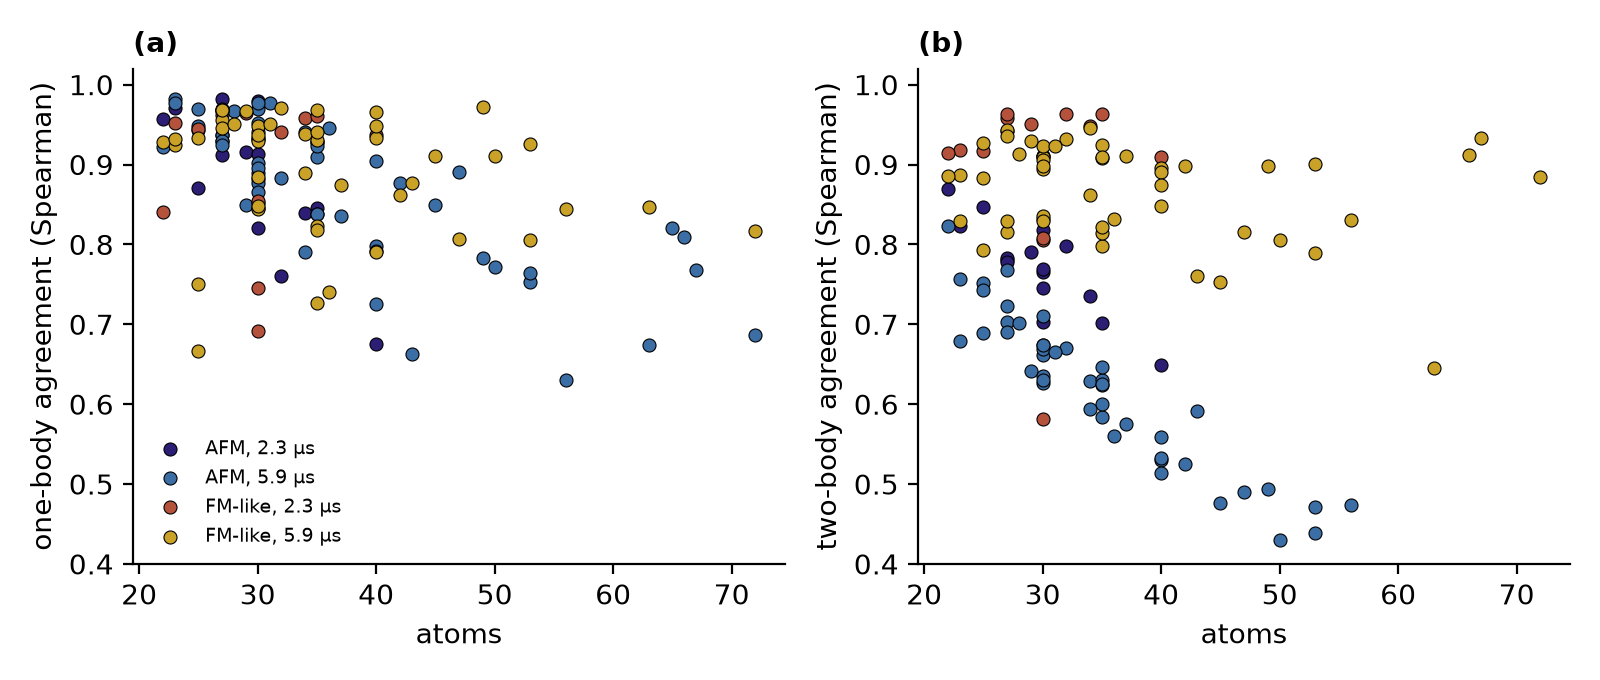
\includegraphics[width=0.95\textwidth]{si_fresnel.png}
\caption{Fresnel against emulation, per job: (a) one-body and (b) two-body Spearman agreement against register size, by drive and pulse length.}
\label{fig:fresnel}
\end{figure}

\renewcommand{\refname}{References}
\bibliographystyle{sn-vancouver-num}
\bibliography{references}
\end{document}
